\documentclass[12pt]{article}
\usepackage{graphicx}
\usepackage{amsmath}
\usepackage{amssymb}
\usepackage{hyperref}
\usepackage{geometry}
\usepackage{cite}
\geometry{a4paper, margin=1in}
\usepackage{array}

\title{
    
\includegraphics[width=0.3\textwidth]{images/UWindsor.jpg} \\[0.5cm]
    \textbf{Project Report} \\[0.5cm]
    \large For \\[0.5cm]
    ELEC-8900-110 Special Topics: Connected Autonomous Vehicles \\
    \normalsize Fall 2024 \\[0.5cm]
    \large \textbf{Real-Time Object Detection and Collision Avoidance} \\[0.5cm]
}

\author{
    \textbf{Submitted To:} \\ 
    Dr. Ning Zhang \\[0.5cm]
    \textbf{Submitted By:} \\[0.5cm]
    \begin{tabular}{|>{\raggedright}p{6cm}|>{\raggedright\arraybackslash}p{6cm}|}
        \hline
        \textbf{Student Name} & \textbf{Student ID} \\
        \hline
        Sakib Sadman Shajib & 110157626 \\
        \hline
        Tabein Rayhan & 110130126 \\
        \hline
        Raunaq Singh Saggu & 110129245 \\
        \hline
    \end{tabular} \\[2cm]
}

\date{\large November 2024}

\begin{document}

% Title page (no page number)
\maketitle
\thispagestyle{empty} % No page number on title page
\newpage

% Roman page numbering for TOC and List of Figures
\pagenumbering{roman}

% Table of contents
\tableofcontents
\newpage

% List of Figures
\listoffigures
\newpage

% Start Arabic numbering from the Introduction
\pagenumbering{arabic}

\begin{abstract}
Real-time object detection and collision avoidance are critical in numerous applications such as autonomous vehicles and robotics. This report provides a comprehensive overview of the implemented AI model, utilizing the YOLOv11 architecture. It includes insights from related research to support the approach, detailing the model's architecture, training methodology, GPU acceleration, performance metrics, and real-world application potential.
\end{abstract}

\section{Introduction}

Real-time object detection and collision avoidance are essential components of modern autonomous systems, including self-driving cars and robotic platforms. The ability to detect objects and avoid collisions in real-time enhances both safety and operational efficiency. This report focuses on the development of a real-time collision avoidance system using a state-of-the-art YOLOv11 model and outlines the use of GPUs for improved performance.

\section{Related Work and Approach}

The existing research on real-time object detection and collision avoidance includes several effective frameworks involving deep learning, sensor-based approaches, and hybrid methods. This report builds upon related research and introduces a refined implementation for improved performance.

\subsection{Stereo and Depth Sensors for Object Detection}
Stereo-camera-based approaches are also well documented, such as Eppenberger et al.'s work \cite{eppenberger2020leveraging} on leveraging stereo data for dynamic obstacle detection and tracking. Xu et al. \cite{xu2022real} also highlight the benefits of combining RGB-D data for autonomous driving and collision avoidance. While our approach does not utilize stereo cameras, these methods offer additional depth perception capabilities useful in cluttered environments.

\subsection{GPU Utilization for Real-Time Computation}
To enhance the real-time capabilities of our system, we leverage GPU-accelerated computations. Bedada and Palli \cite{bedada2024real} demonstrated the use of GPU-computed distance maps for real-time collision avoidance, significantly improving the responsiveness of robotic platforms. We adopt a similar GPU-centric approach for training and inference, utilizing NVIDIA Tesla P100 for model training and NVIDIA GTX 1060 Laptop for inference to achieve fast processing speeds.

\subsection{Vision Transformer for Collision Avoidance}
Recent advancements like the V-CAS framework by Ashraf et al. \cite{ashraf2024v} utilize vision transformers for real-time collision avoidance using multi-camera streams. Although we opted for the YOLOv11 model due to its lightweight architecture and suitability for constrained environments, vision transformers represent a promising direction for future work involving higher computational resources.

\subsection{Obstacle Detection and Tracking in Urban Environments}
Urmson et al. \cite{urmson2008autonomous} and Darms et al. \cite{darms2008obstacle} demonstrated advanced systems for obstacle detection and tracking in urban environments, focusing on autonomous vehicle performance. Their work highlights the importance of integrating multiple sensors and advanced tracking algorithms, which inspired elements of our object detection and avoidance approach.

\section{Model Architecture}

The core of our real-time object detection system is the YOLOv11 architecture. YOLOv11 is known for its speed and accuracy, which makes it suitable for real-time applications. The model uses:

\begin{itemize}
    \item \textbf{C3K2 blocks}: These blocks are used for efficient feature extraction, enabling the model to identify complex and small objects effectively.
    \item \textbf{C2PSA (Cross-Channel Pyramid Self-Attention)}: This mechanism ensures that the model focuses computational resources on significant image regions, optimizing detection accuracy \cite{ashraf2024v}.
\end{itemize}

The YOLOv11 architecture is an advancement over its predecessors, employing residual connections and DenseNet-inspired modules to ensure optimal feature propagation and reduce redundancy. The head of the network supports multi-scale prediction layers, which allows for detecting objects at varying scales.

\section{Training and Dataset Preparation}

\subsection{Dataset Preparation}
The training dataset includes labeled images representing various operational environments, as shown in Figure \ref{fig:training_dataset}. We utilized the KITTI dataset for cars and custom datasets tailored for autonomous driving scenarios. These datasets were annotated with bounding boxes for different object classes, as shown in Figure \ref{fig:label_correlogram}. The frequency and spatial distribution of these labels are shown in Figure \ref{fig:label_distribution}. KITTI is particularly useful for autonomous driving applications due to its diverse set of images from urban and semi-urban environments \cite{xu2022real}.

\section{Training and Dataset Preparation}

% Training Dataset Image
\begin{figure}[h]
    \centering
    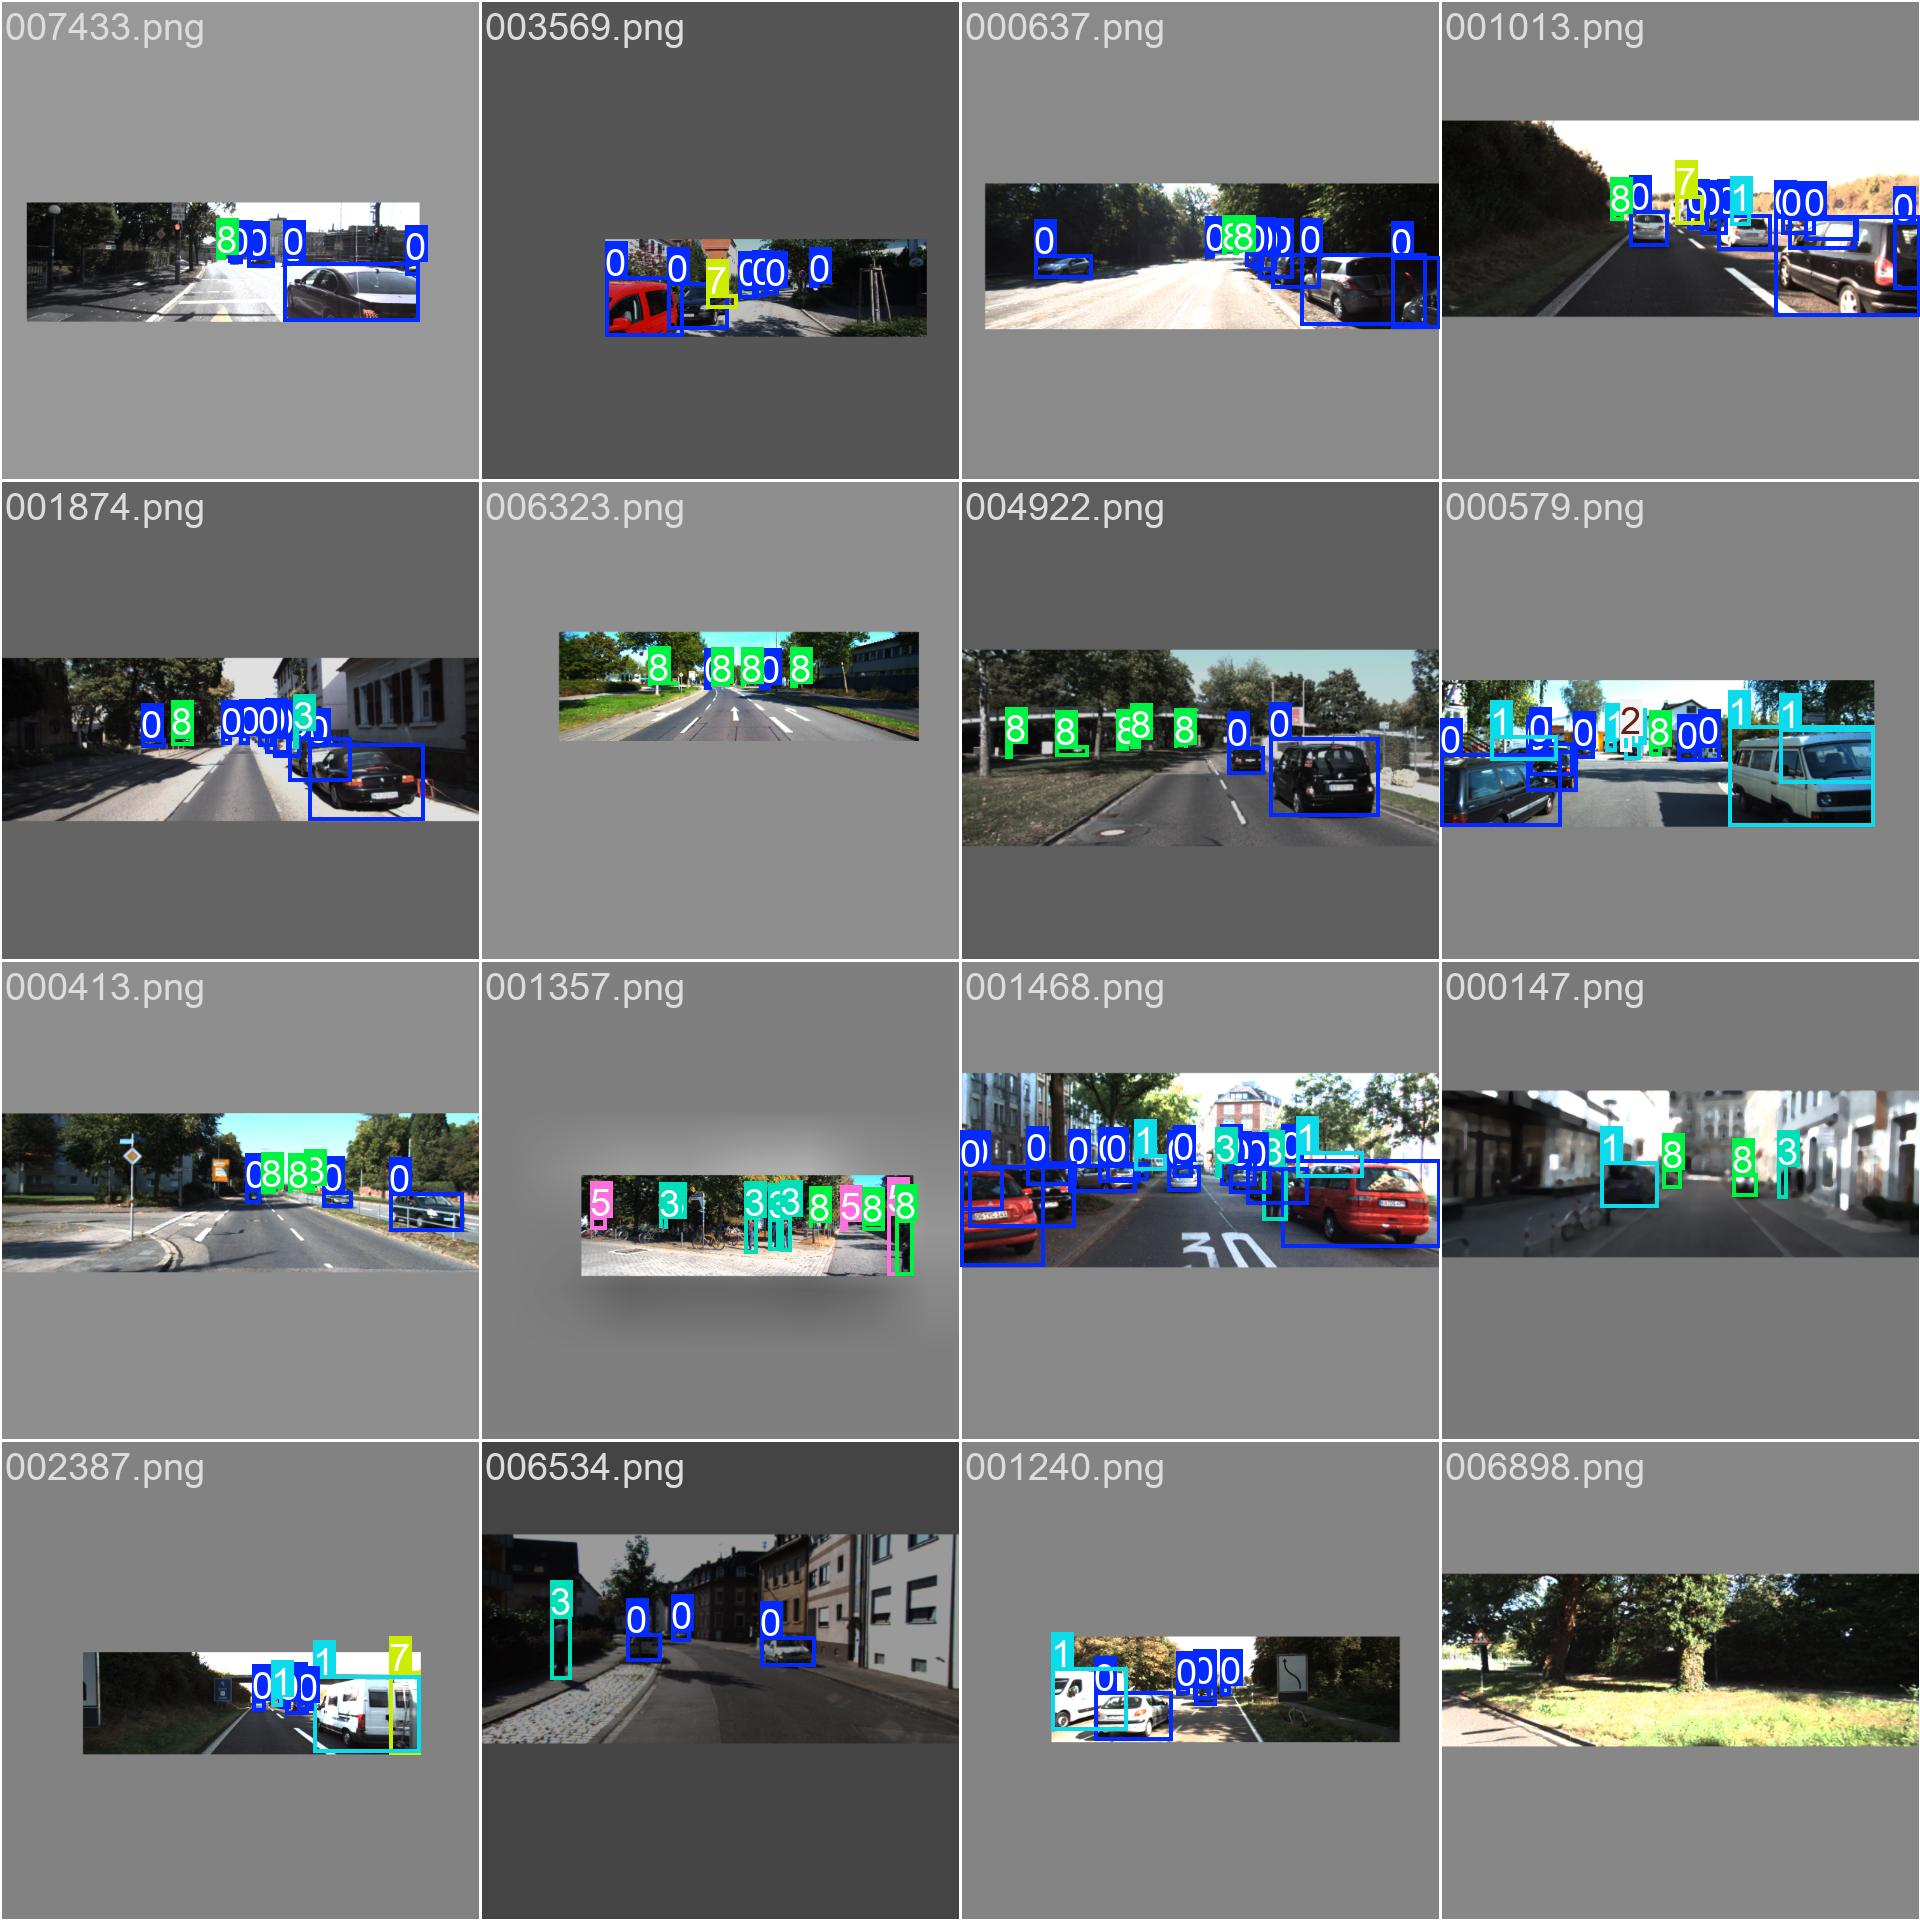
\includegraphics[width=\textwidth]{images/train_batch16842.jpg}
    \caption{Training images showing bounding boxes and labels for different object classes, illustrating dataset diversity and annotation quality.}
    \label{fig:training_dataset}
\end{figure}

% Label Distribution Image
\begin{figure}[h]
    \centering
    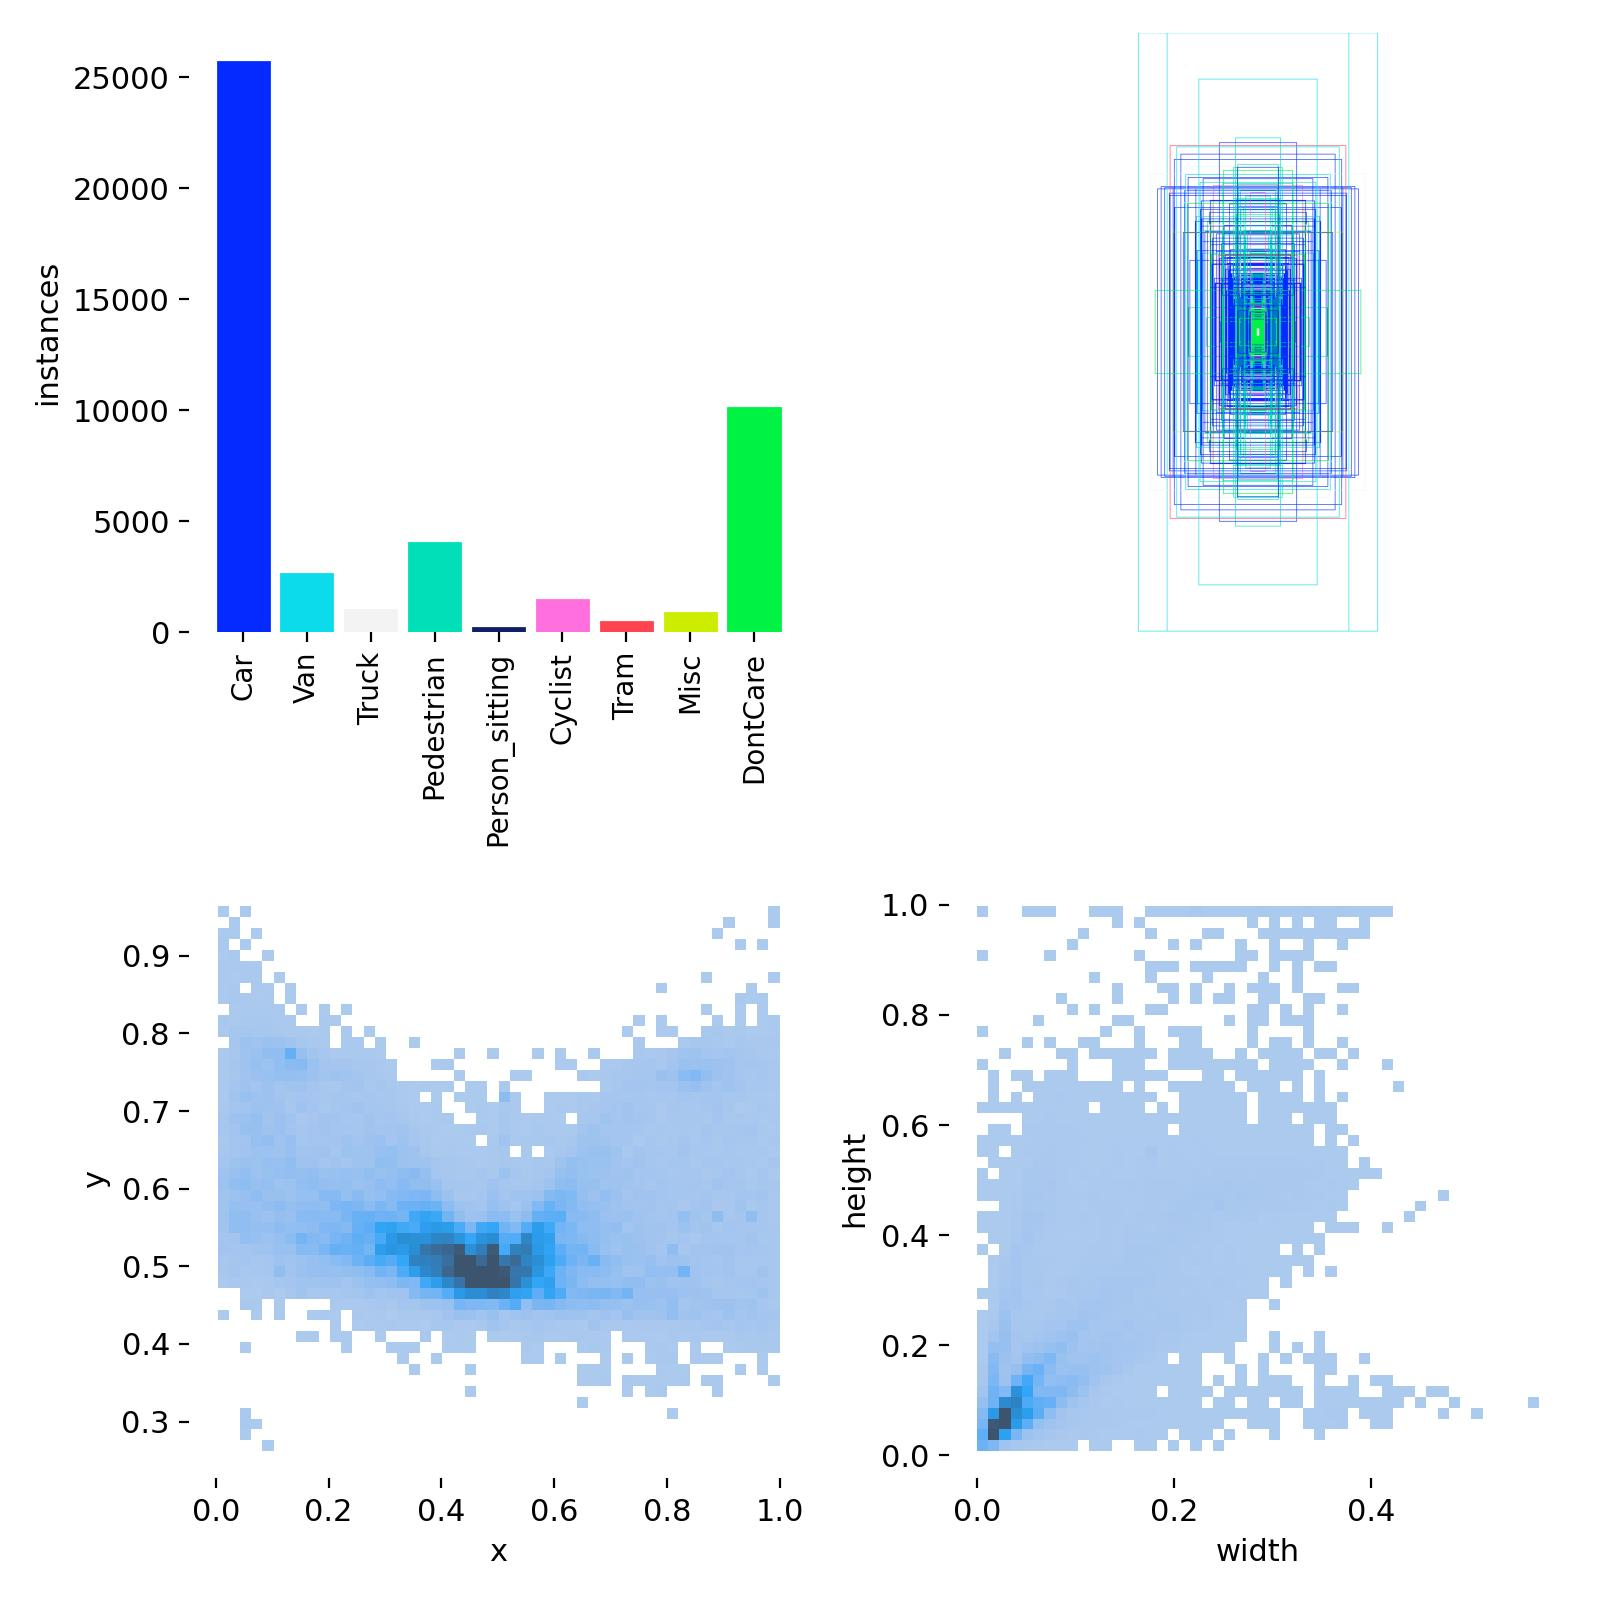
\includegraphics[width=\textwidth]{images/labels.jpg}
    \caption{Frequency and spatial distribution of labeled objects in the dataset.}
    \label{fig:label_distribution}
\end{figure}

% Label Correlogram Image
\begin{figure}[h]
    \centering
    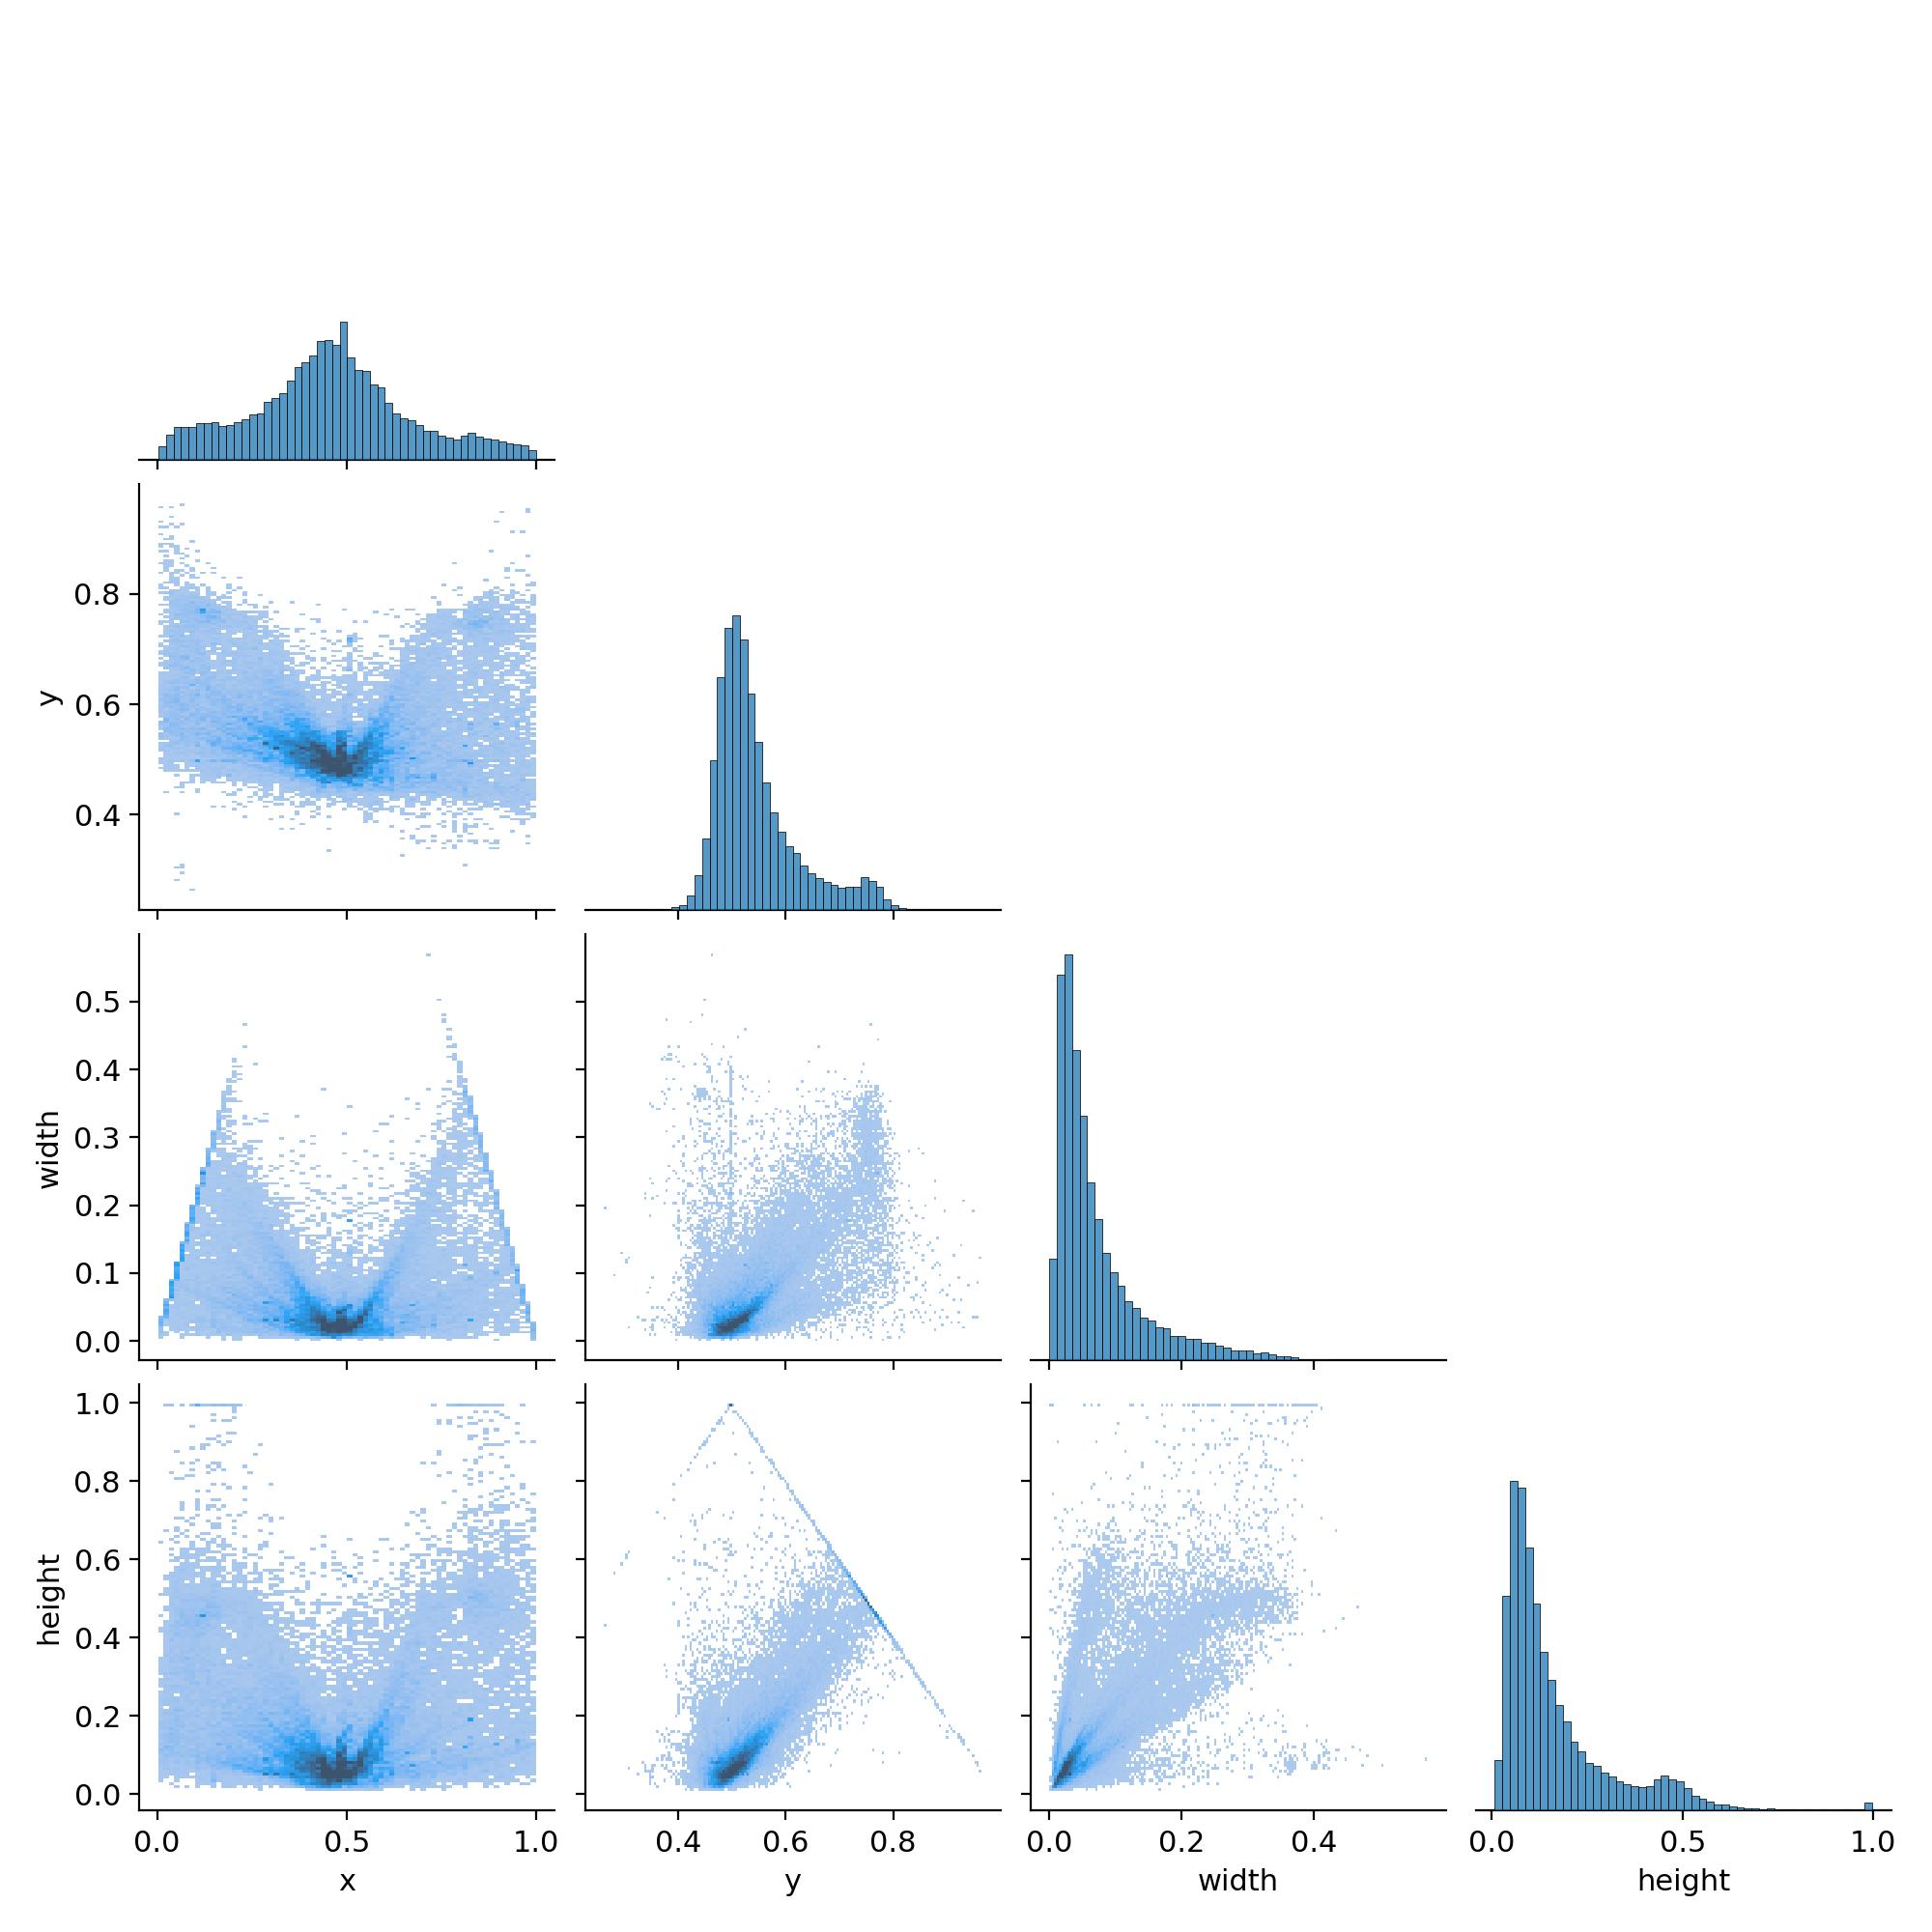
\includegraphics[width=\textwidth]{images/labels_correlogram.jpg}
    \caption{Correlogram showing relationships between label attributes such as bounding box width and height.}
    \label{fig:label_correlogram}
\end{figure}


\subsection{Training Strategy}
We used stochastic gradient descent (SGD) with momentum for training. A learning rate scheduler adjusted the learning rate dynamically throughout the training process. Training was conducted over 50 epochs, with early stopping based on validation loss to mitigate overfitting. Data augmentation techniques—such as random flips, rotations, and color jittering—were applied to improve model robustness \cite{li2022real}.

GPU acceleration played a key role in reducing training time. The model was trained using an NVIDIA Tesla P100 GPU, allowing for efficient computation of the extensive batch matrices involved in convolutional operations. Additionally, batch size and image size were optimized for training, striking a balance between computational load and performance. Figure \ref{fig:training_performance} shows the training and validation losses, as well as other key performance metrics across training epochs.

\section{Performance Metrics and Evaluation}

To evaluate the model, we employed metrics such as precision (P), recall (R), mean Average Precision at IoU threshold 0.50 (mAP50), and mean Average Precision averaged over IoU thresholds from 0.50 to 0.95 (mAP50-95). The validation predictions of the model are illustrated in Figure \ref{fig:validation_predictions}. YOLOv11 achieved the following results on our test dataset:

\begin{itemize}
    \item \textbf{Precision (P)}: 0.87
    \item \textbf{Recall (R)}: 0.786
    \item \textbf{mAP50}: 0.841
    \item \textbf{mAP50-95}: 0.617
\end{itemize}

FPS was recorded at 14.43 on an NVIDIA GTX 1060 Laptop, making the system suitable for real-time applications \cite{ashraf2024v}.

\section{Performance Metrics and Evaluation}

% Validation Predictions Image
\begin{figure}[h]
    \centering
    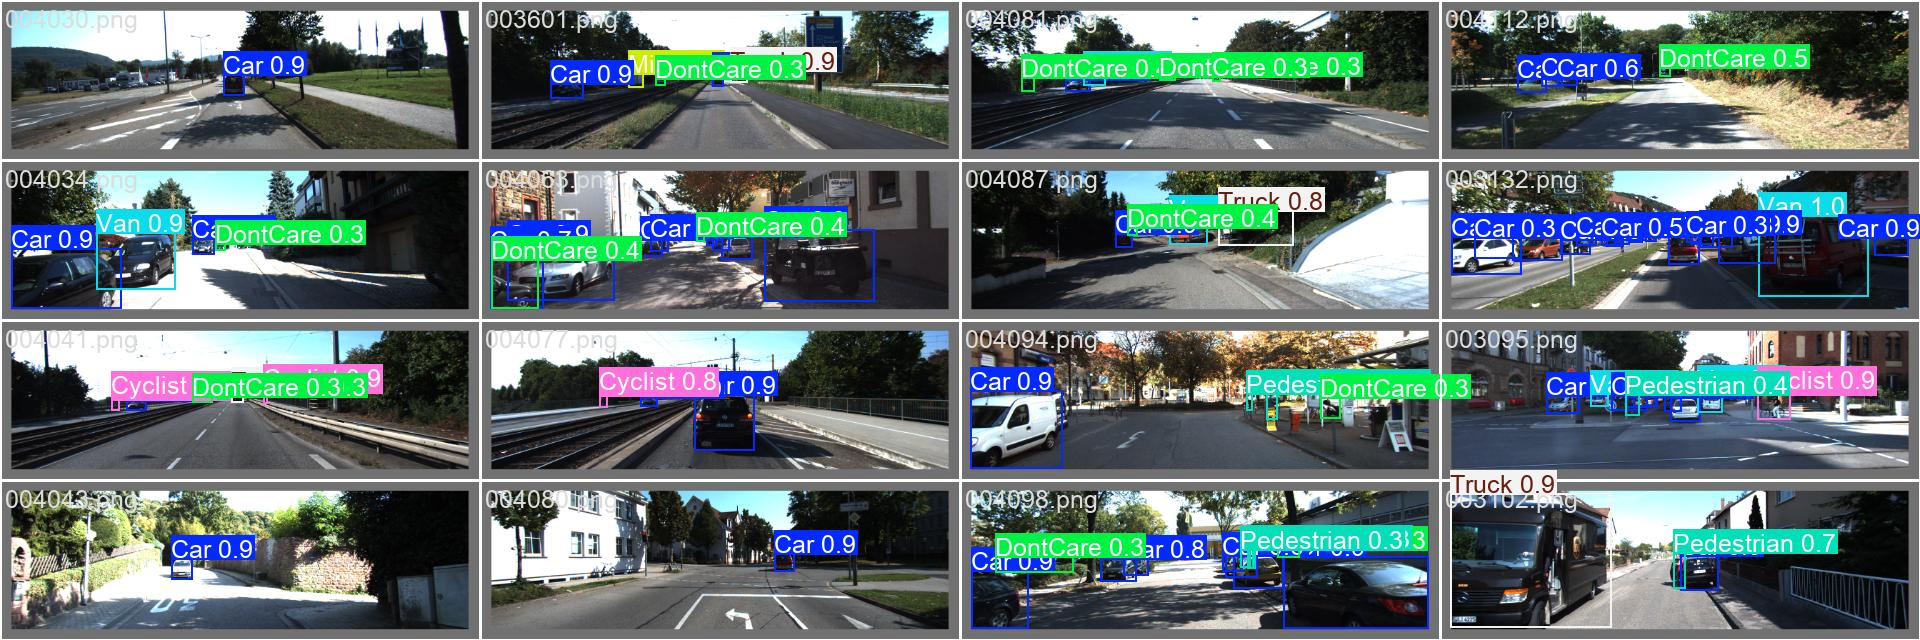
\includegraphics[width=\textwidth]{images/val_batch2_pred.jpg}
    \caption{Validation set predictions with bounding boxes and confidence scores, showing the performance of YOLOv11 on real-world validation images.}
    \label{fig:validation_predictions}
\end{figure}

% Training Performance Trends Image
\begin{figure}[h]
    \centering
    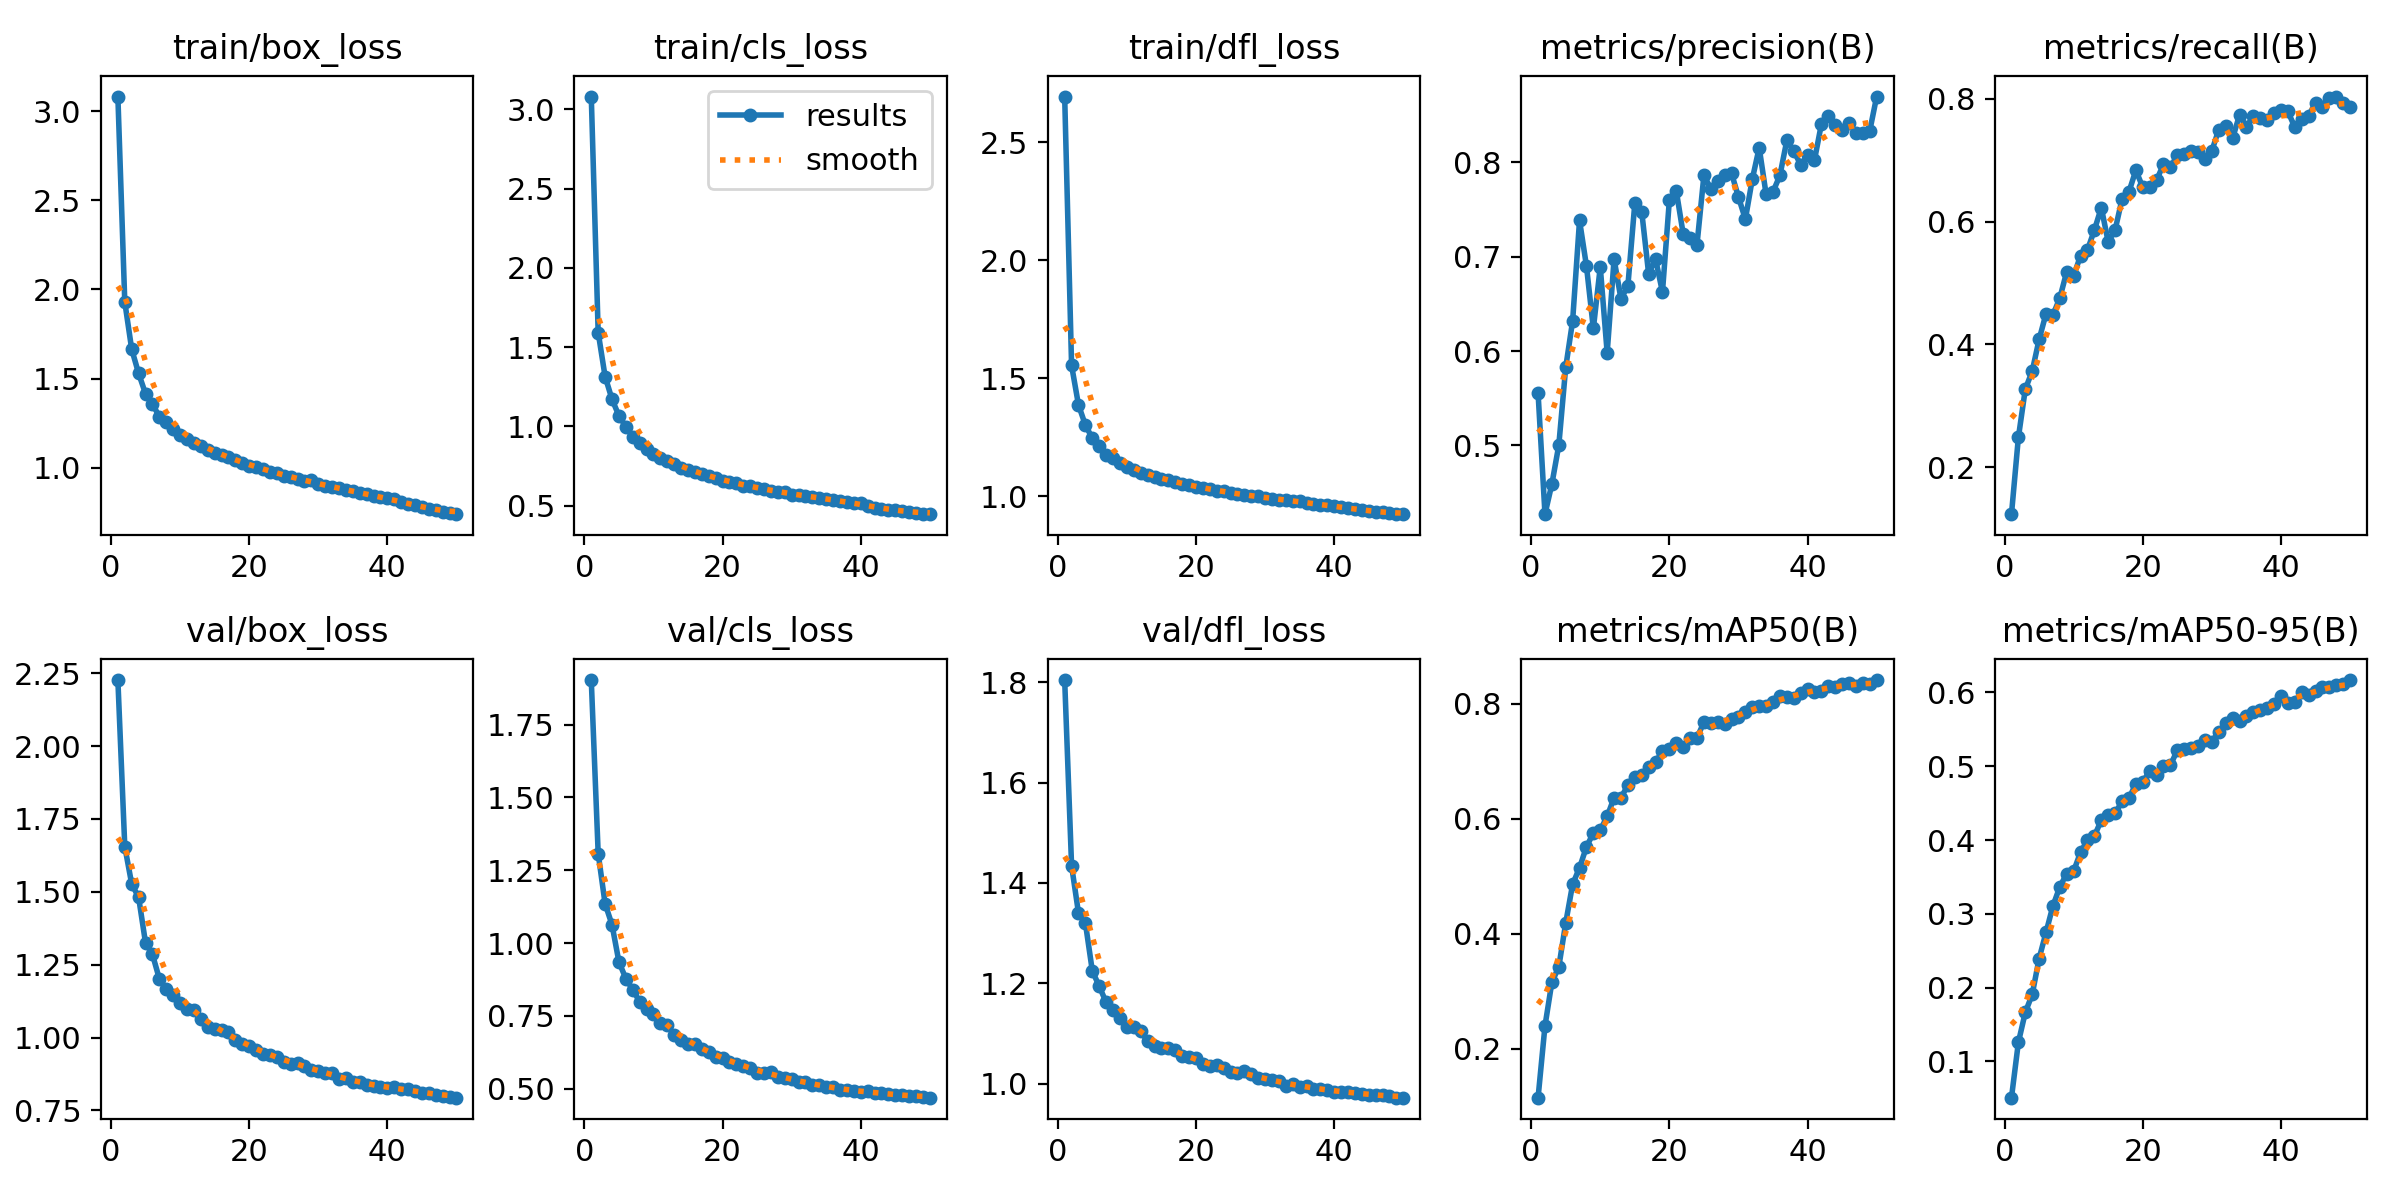
\includegraphics[width=\textwidth]{images/results.png}
    \caption{Training and validation losses, precision, recall, mAP, and other metrics over training epochs.}
    \label{fig:training_performance}
\end{figure}

\subsection{Evaluation Metrics}

% Recall-Confidence Curve Image
\begin{figure}[h]
    \centering
    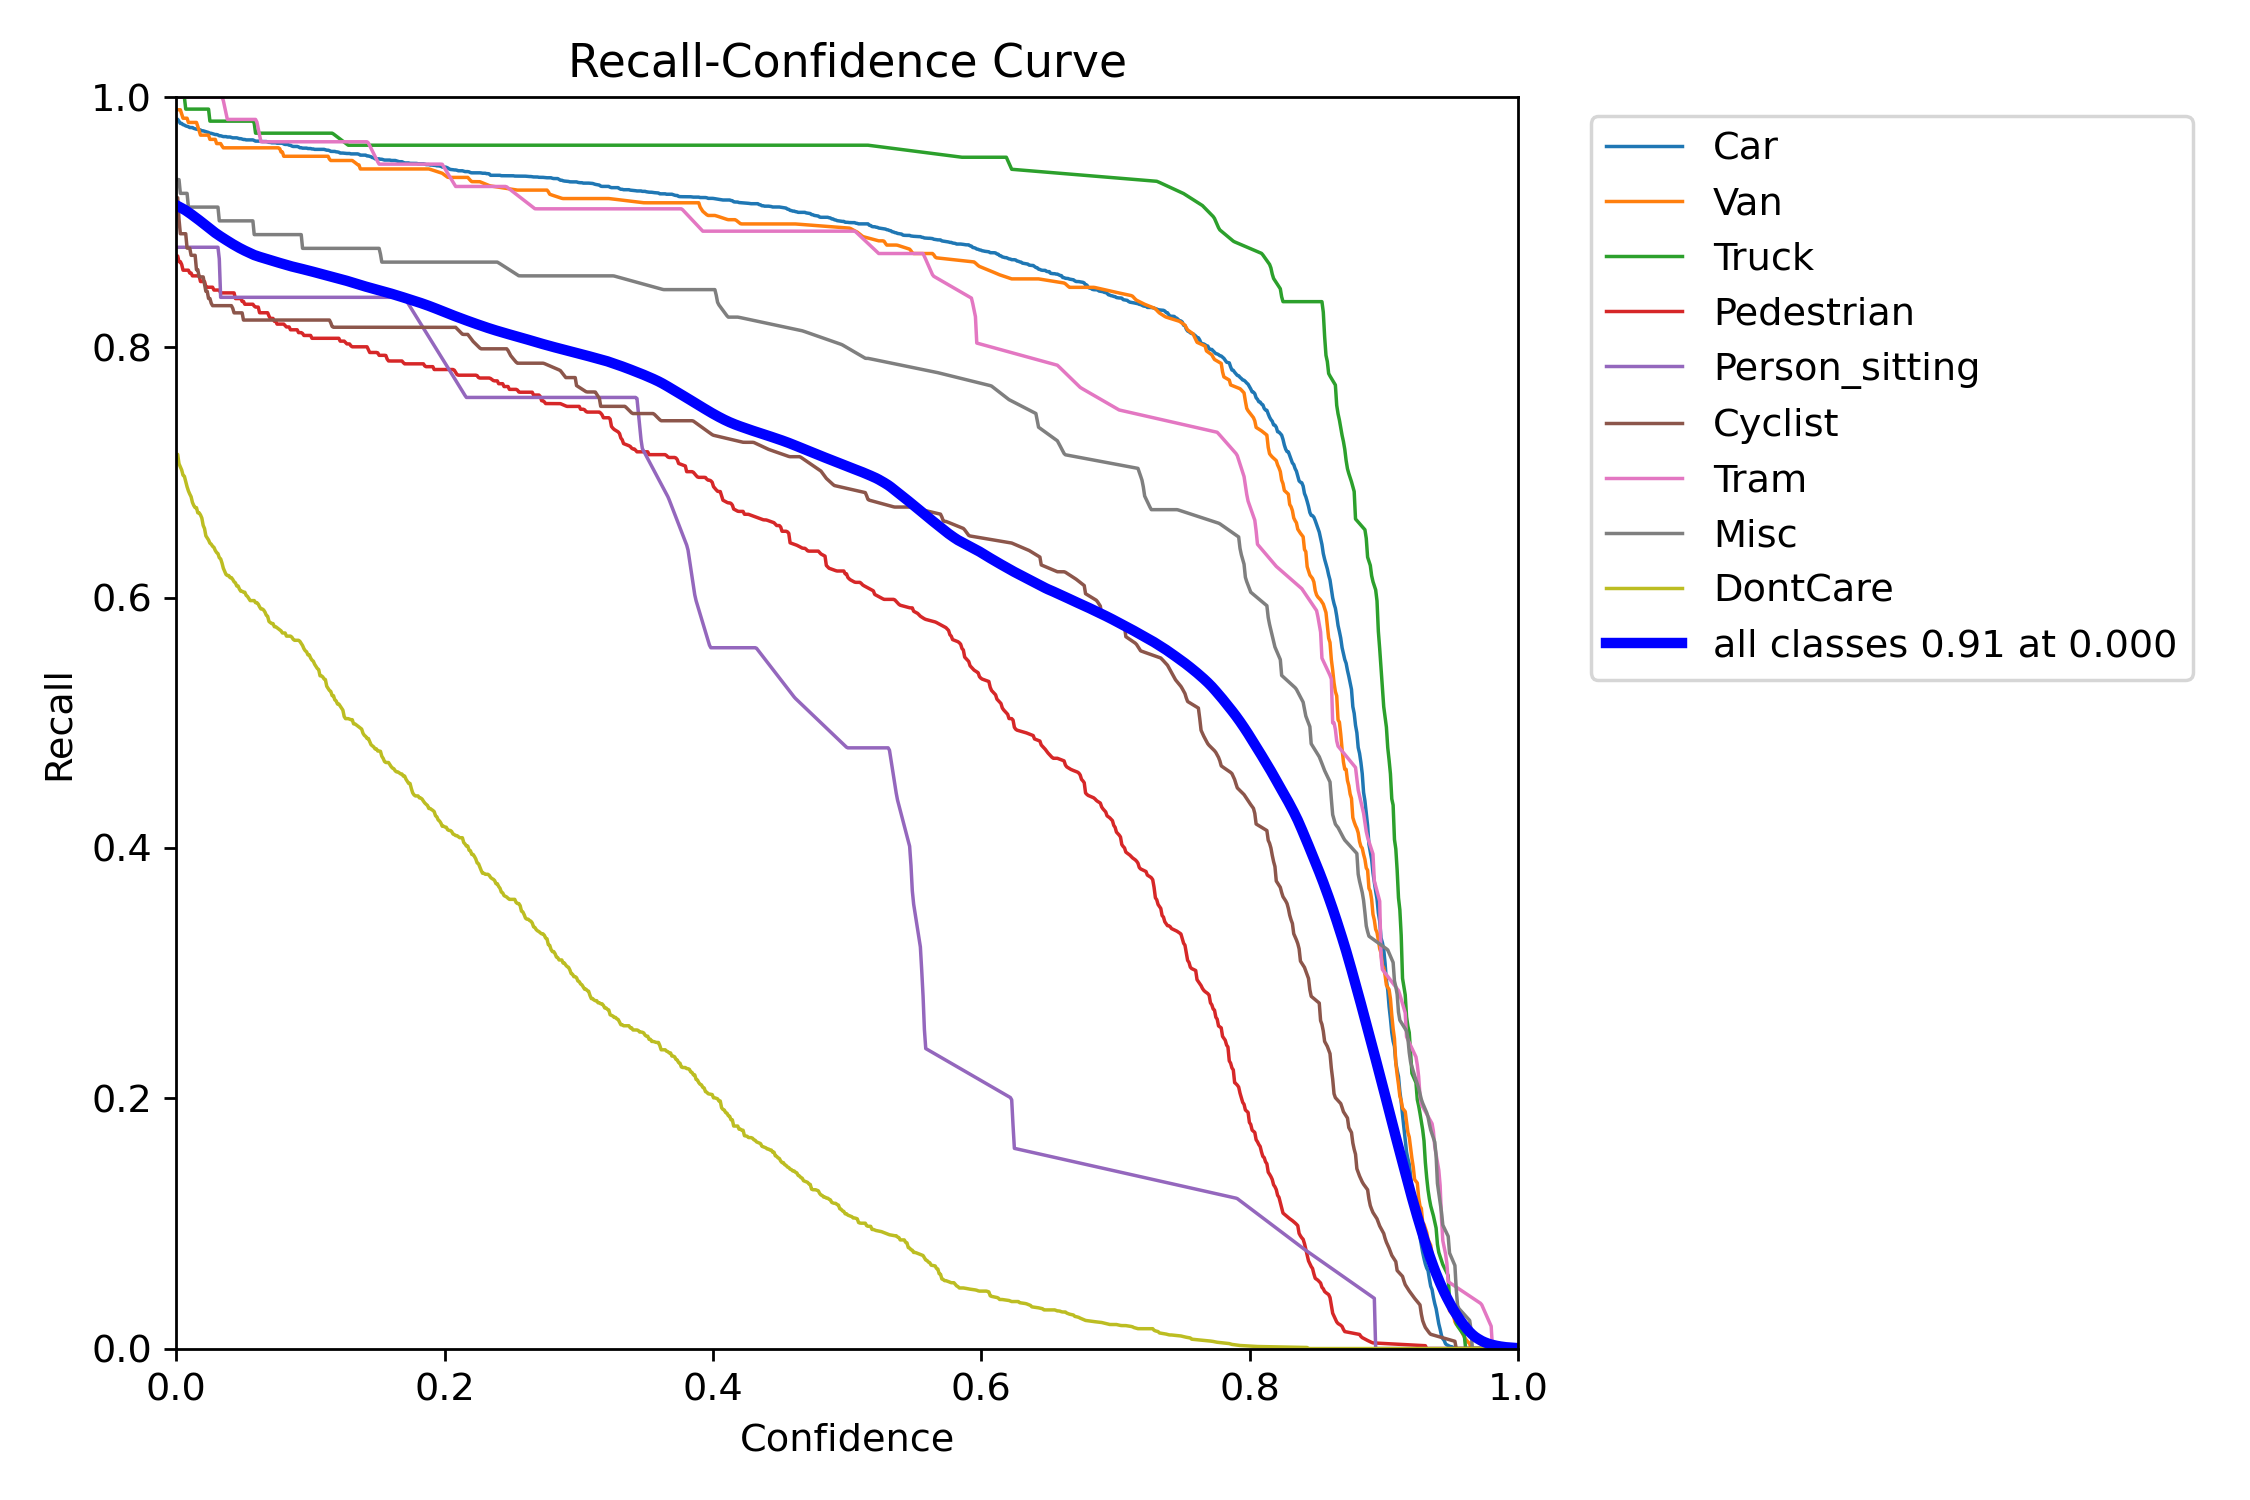
\includegraphics[width=\textwidth]{images/R_curve.png}
    \caption{Recall-Confidence curve showing the relationship between confidence thresholds and recall for different object classes.}
    \label{fig:recall_confidence_curve}
\end{figure}

% Precision-Recall Curve Image
\begin{figure}[h]
    \centering
    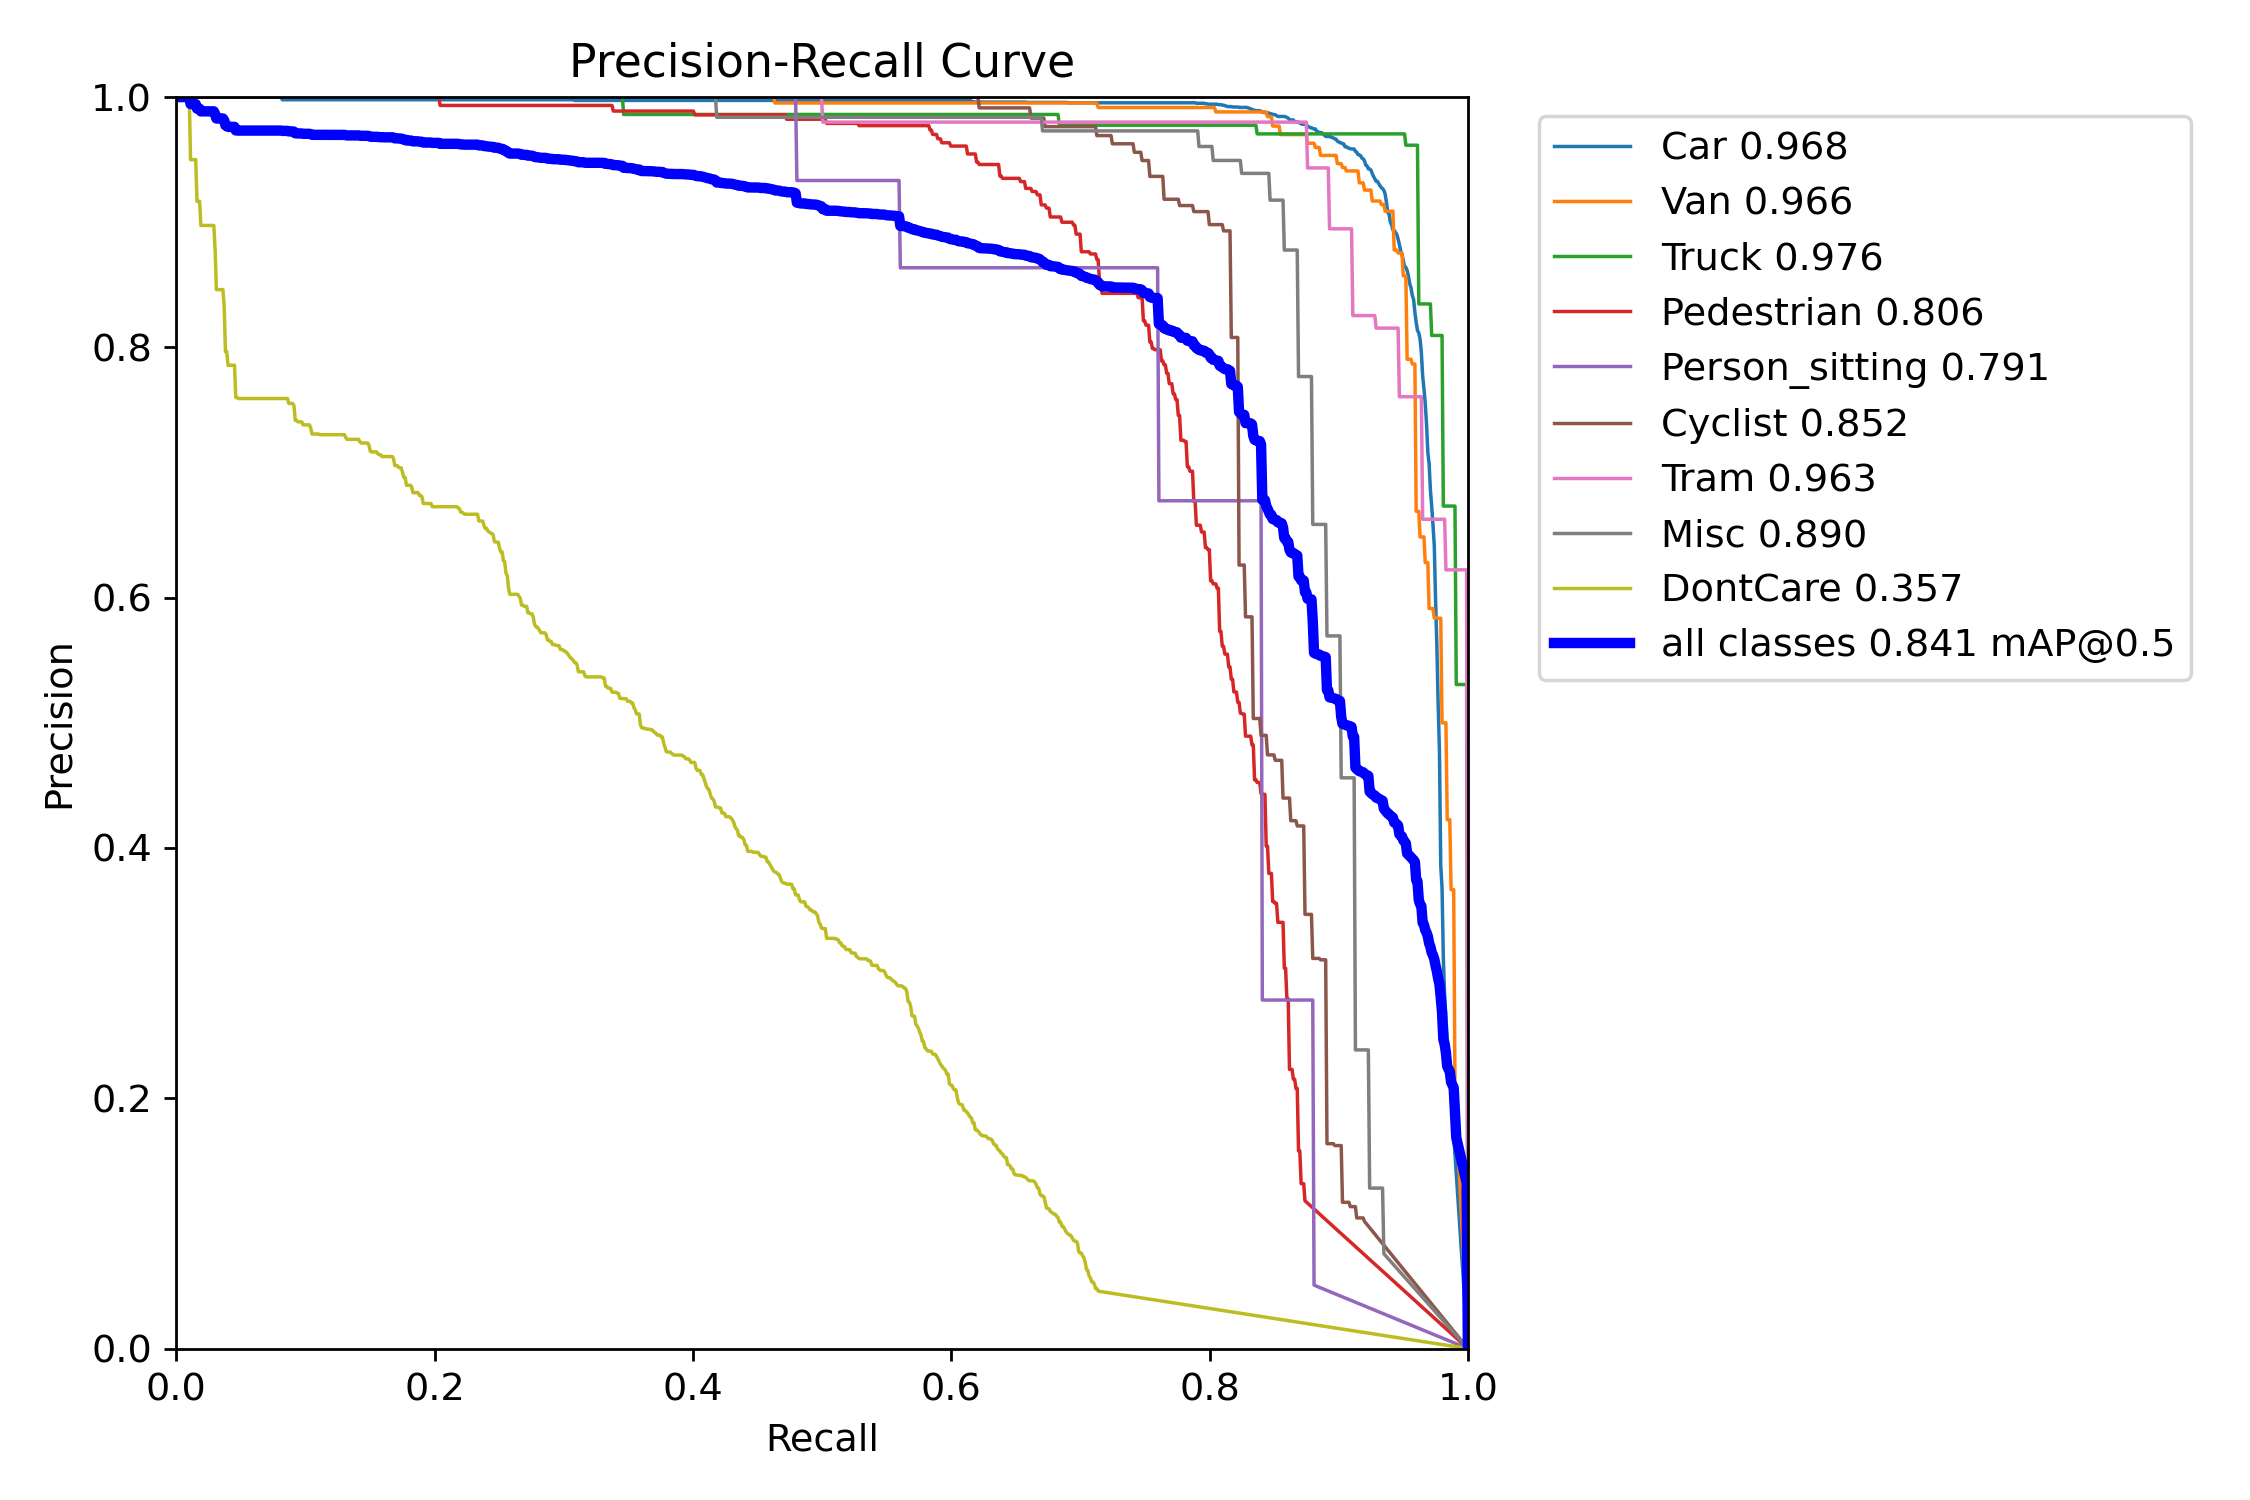
\includegraphics[width=\textwidth]{images/PR_curve.png}
    \caption{Precision-Recall curve illustrating the trade-off between precision and recall for different confidence thresholds.}
    \label{fig:precision_recall_curve}
\end{figure}

% Precision-Confidence Curve Image
\begin{figure}[h]
    \centering
    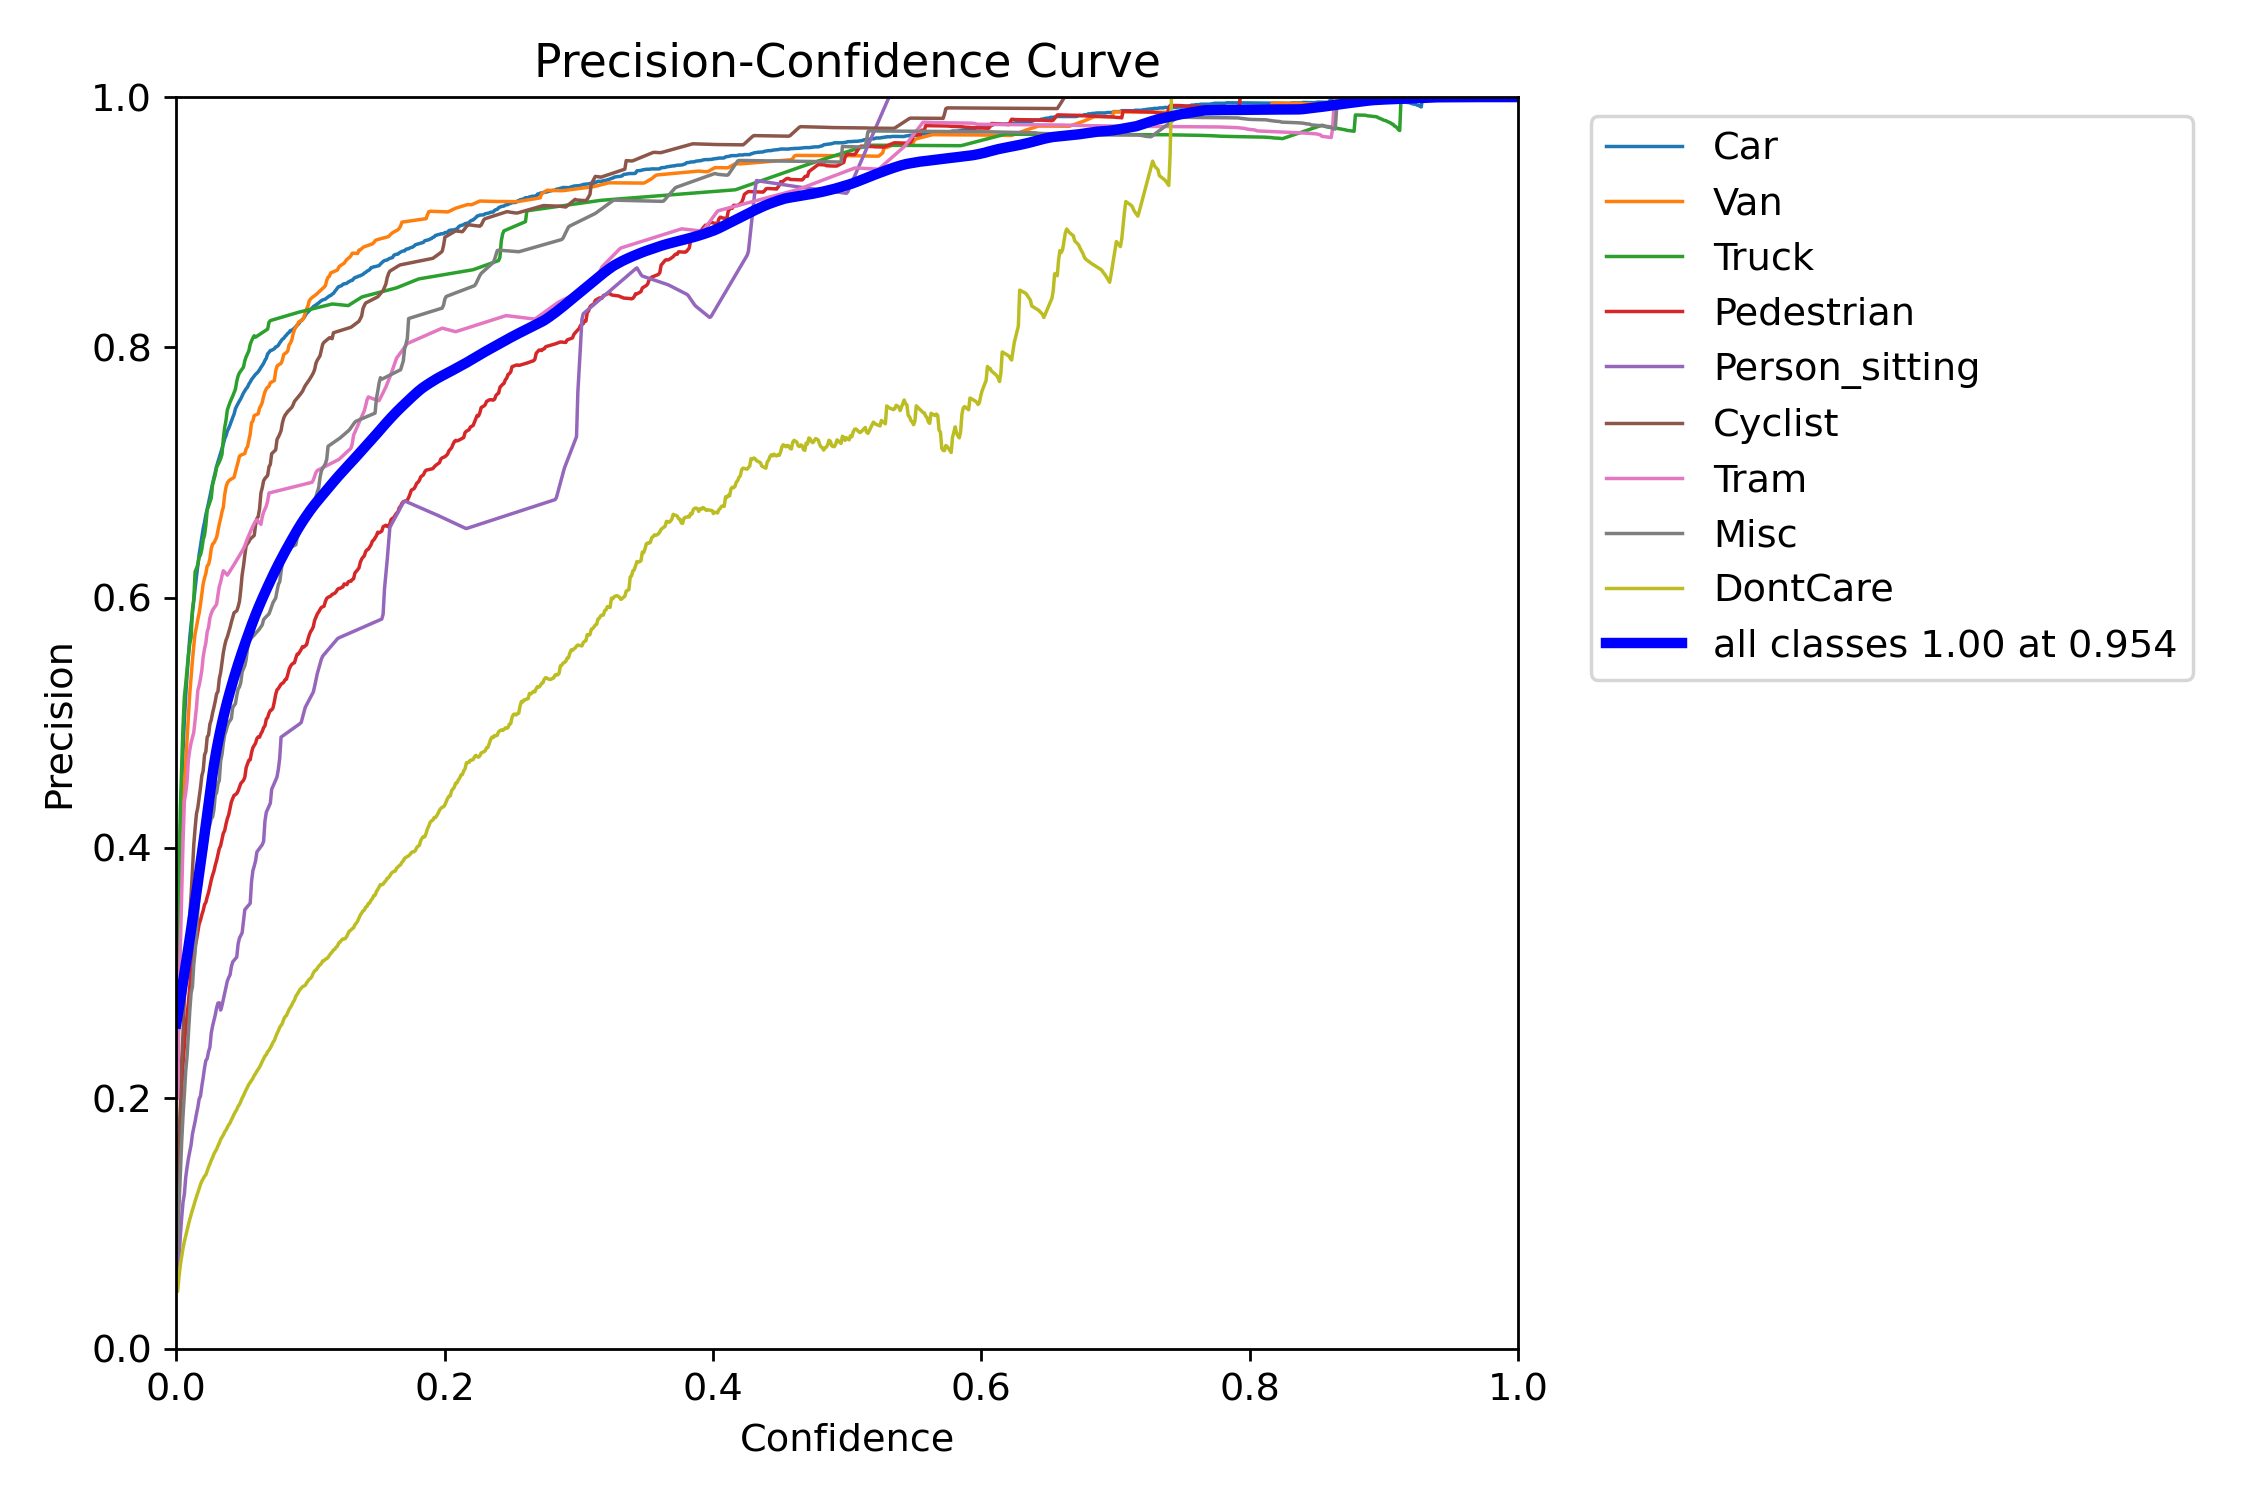
\includegraphics[width=\textwidth]{images/P_curve.png}
    \caption{Precision-Confidence curve showing precision across different confidence thresholds for all object classes.}
    \label{fig:precision_confidence_curve}
\end{figure}

% F1-Confidence Curve Image
\begin{figure}[h]
    \centering
    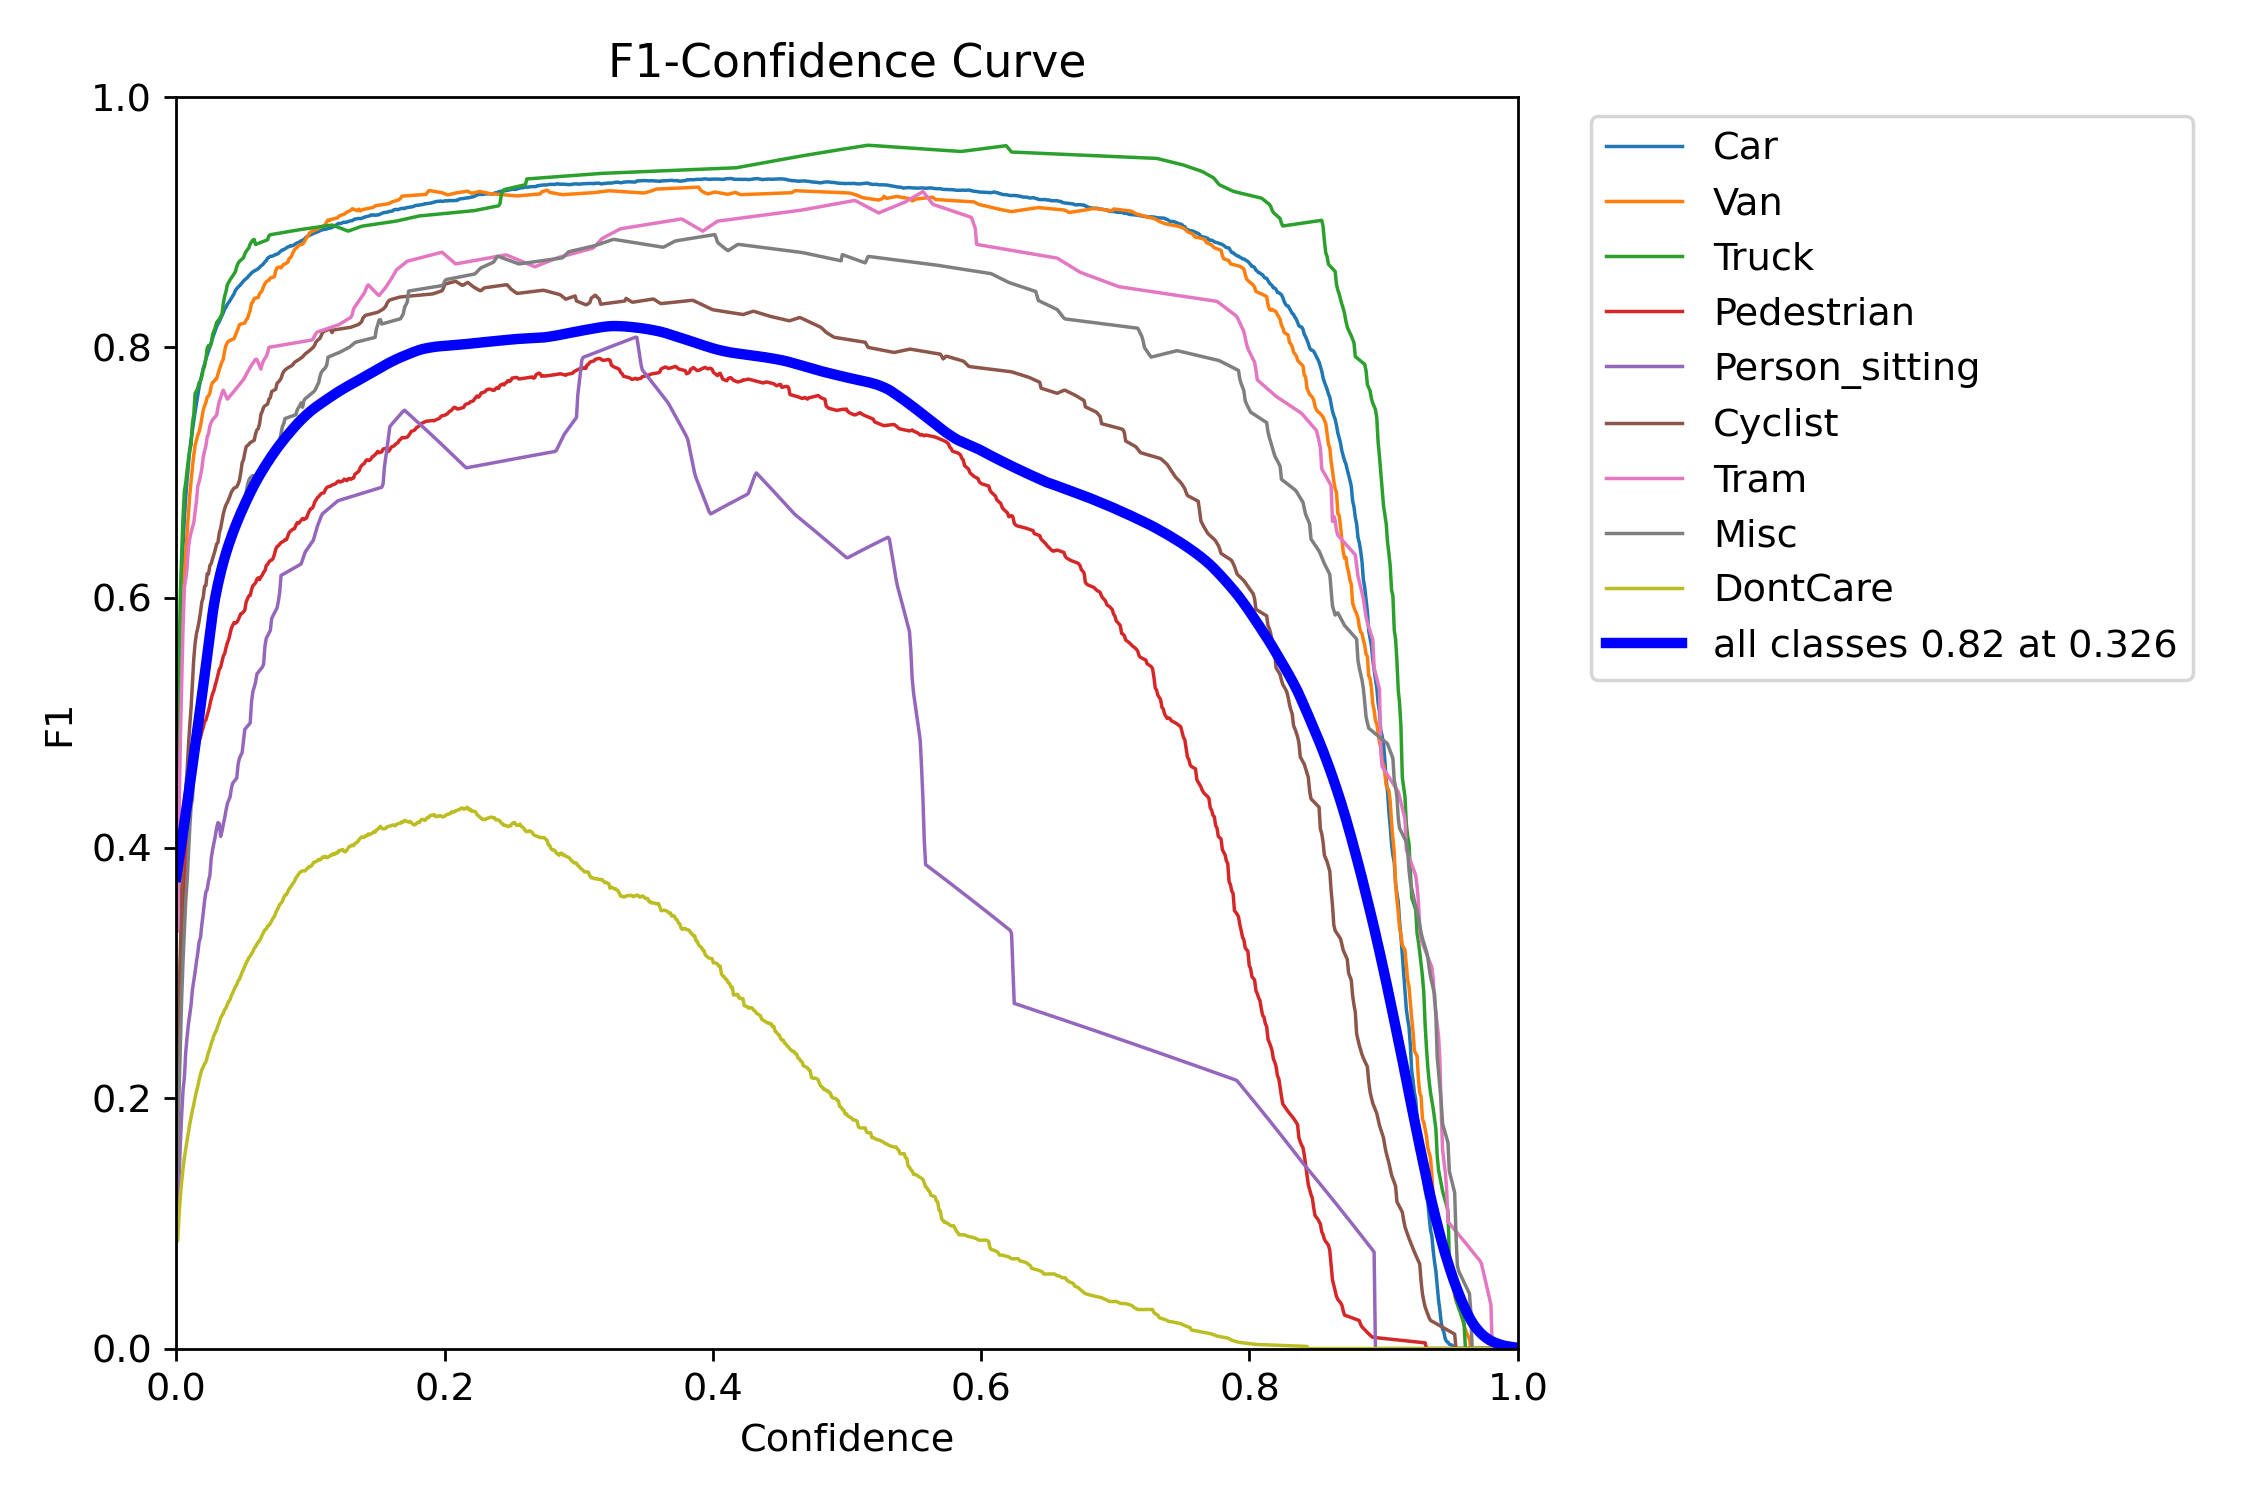
\includegraphics[width=\textwidth]{images/F1_curve.png}
    \caption{F1-Confidence curve displaying the balance between precision and recall for different confidence thresholds.}
    \label{fig:f1_confidence_curve}
\end{figure}

% Confusion Matrix Image
\begin{figure}[h]
    \centering
    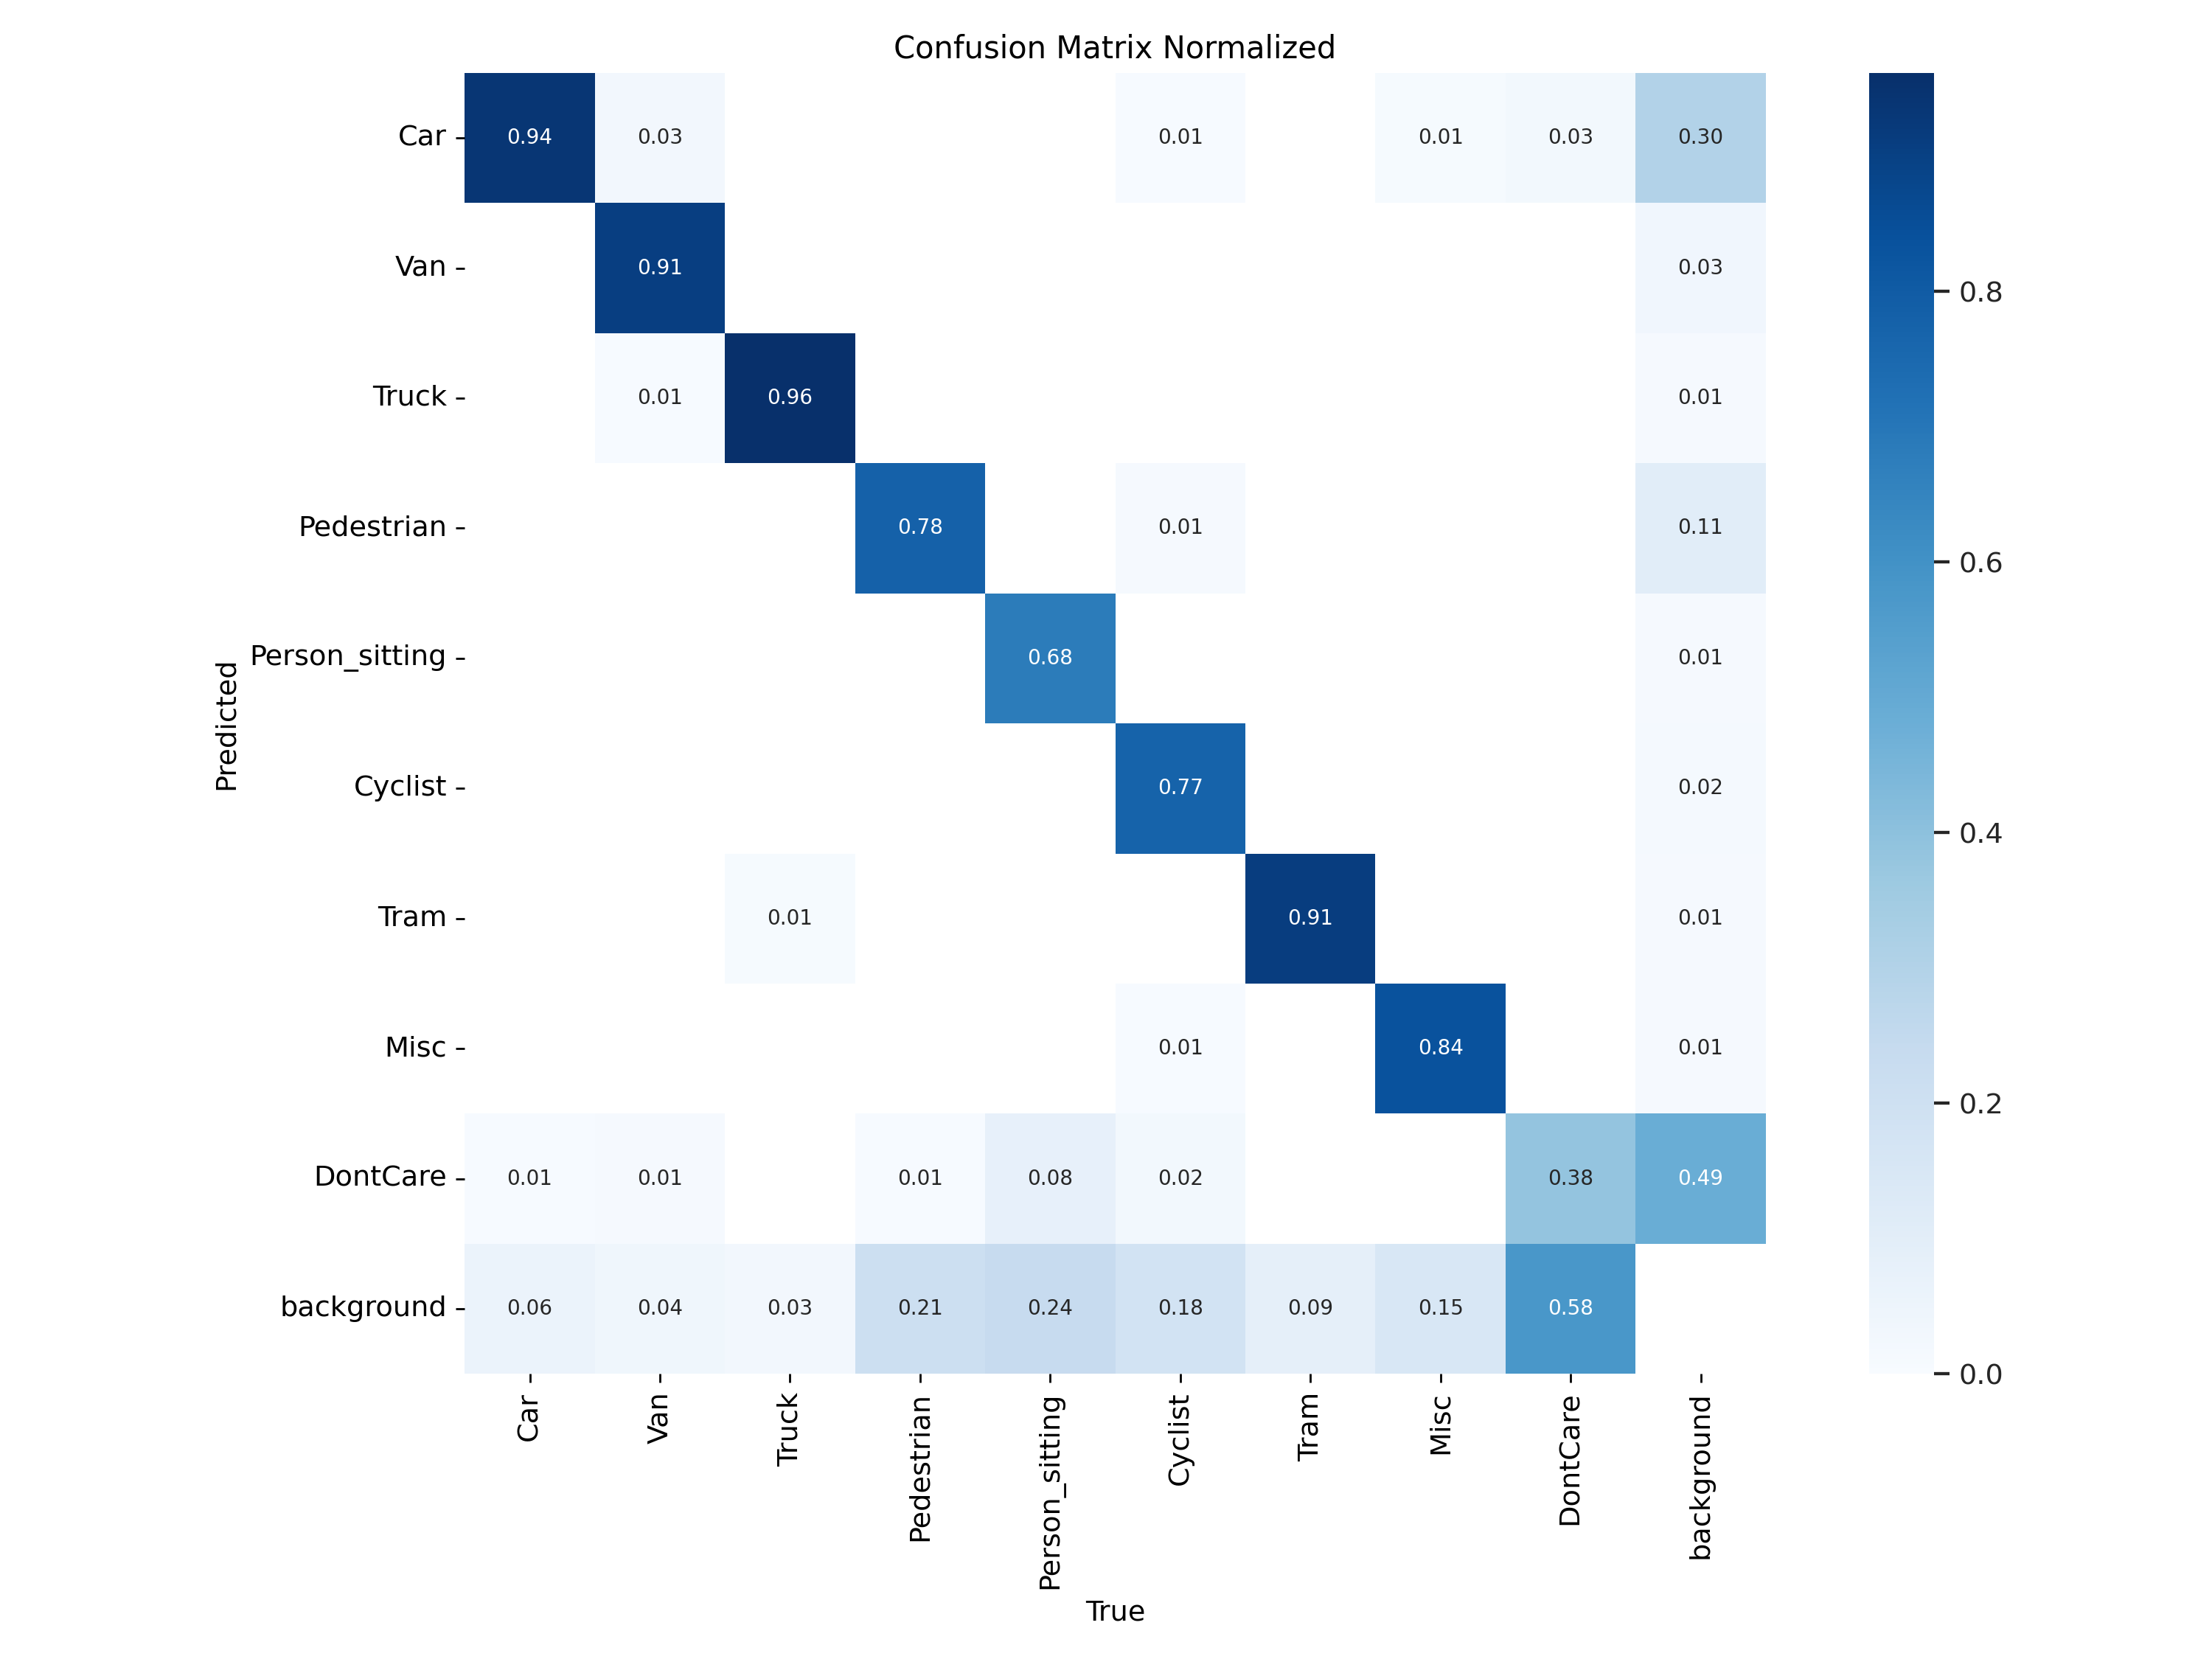
\includegraphics[width=\textwidth]{images/confusion_matrix_normalized.png}
    \caption{Normalized confusion matrix visualizing the model's performance in classifying objects.}
    \label{fig:confusion_matrix}
\end{figure}

The results showed high precision across various recall values, highlighting the model's reliability even under challenging conditions, such as low light or partial occlusion scenarios \cite{eppenberger2020leveraging}. Figures \ref{fig:recall_confidence_curve}, \ref{fig:precision_recall_curve}, \ref{fig:precision_confidence_curve}, and \ref{fig:f1_confidence_curve} illustrate the recall-confidence, precision-recall, precision-confidence, and F1-confidence curves, respectively, that were used to evaluate the model's performance.

\section{Collision Avoidance System}

Effective collision avoidance necessitates real-time perception based on detected objects. Our approach utilizes the YOLOv11 model to detect obstacles in real time and generate appropriate avoidance actions.

\subsection{Ultrasonic-Based Object Detection}
In environments where vision-based systems might fail, such as due to lighting conditions, low-cost ultrasonic sensors have proven to be a reliable alternative for collision detection. Yasin et al. \cite{yasin2020low} demonstrated effective usage of ultrasonic sensors for autonomous robots, which complements our approach in certain challenging conditions.

\section{Practical Application}
The GPU acceleration of the detection model facilitates rapid reactivity, crucial in autonomous vehicles. Similar to the implementation described by Wettergreen et al. \cite{wettergreen2005sun}, our system is designed to operate under dynamic real-world conditions, optimizing detection for efficient energy utilization.

The integration of visual perception from YOLOv11 enables real-time navigation and collision avoidance, particularly for ground vehicles \cite{whittaker2001robotic}. The confusion matrix for classification accuracy is shown in Figure \ref{fig:confusion_matrix}. This combination has been instrumental in reducing computational latency, enabling rapid responses to new obstacles.

\section{Conclusion}

This report presented a comprehensive real-time object detection and collision avoidance system built using YOLOv11 and GPU-accelerated detection. The integration of GPU-based training and inference significantly enhances model efficiency, making it suitable for applications across autonomous vehicles and robotics.

The system achieves a balance between high detection accuracy and real-time performance, allowing it to operate effectively in challenging environments. Future work will aim to incorporate advanced reinforcement learning strategies and explore sensor fusion to further improve the robustness and versatility of collision avoidance capabilities. The use of vision-based and hybrid sensor systems, as discussed by Urmson et al. \cite{urmson2006robust}, represents a promising direction for enhancing autonomy in terrestrial platforms.

\newpage
\appendix
\section{Links}

For further details, please refer to the following links:

\begin{itemize}
    \item Kaggle Notebook: \href{https://www.kaggle.com/code/sakibsadmanshajib/cav-object-detection/}{\texttt{Kaggle Notebook}}
    \item GitHub Repository: \href{https://github.com/sakibsadmanshajib/Real-Time-Object-Detection-for-Collision-Avoidance}{\texttt{GitHub Repository}}
\end{itemize}

\newpage
\bibliographystyle{ieeetr}
\bibliography{references}

\end{document}
